\documentclass[10pt,draftclsnofoot,onecolumn,journal,compsoc]{IEEEtran}
% for IEEEtran usage, see http://www.texdoc.net/texmf-dist/doc/latex/IEEEtran/IEEEtran_HOWTO.pdf

\usepackage[margin=0.75in]{geometry}
\usepackage{graphicx}
\usepackage{caption}
\usepackage{hyperref}
\usepackage{enumerate}
\usepackage[dvipsnames]{xcolor}
\usepackage{amssymb}
\usepackage{listings}
\usepackage{float}
\title{I/O in Linux, FreeBSD, and Windows}
\author{
  \IEEEauthorblockN{Heidi Clayton} \\
  \IEEEauthorblockA{CS 444: Operating Systems II Spring 2017 \\ Oregon State University}
}

\lstdefinestyle{C_listing}{
  language=C,
  keywordstyle=\color{Fuchsia},
  commentstyle=\itshape\color{ForestGreen},
}
\lstset{style=C_listing}


   
\begin{document}
\maketitle
\newpage
\tableofcontents
\newpage
\section{Introduction}
I/O schedulers manage block devices' request queues. They decide the order of insertion and dispatching, and occasionally merges requests together to reduce the overhead of dispatching multiple separate requests \cite{linux1}.

\section{Linux}
Character devices are just a stream of data that is read byte-by-byte. Character devices are simple to schedule since they should just go FIFO. For example, a keyboard is a character device. If you type 'bar', you want 'bar' to be input to the screen in that order, not 'rba' or another combination. It is because of this simplicity that character devices do not have a complicated system for management like block devices do, as described below. \cite{linux1}

In the Linux kernel 2.4, the default scheduler was the Linus Elevator. This has been widely regarded as a fairly mediocre scheduler, as it can often just turn into a FIFO for long periods due to how it handles requests that are considered 'old'. The Linux kernel 2.6 has three built-in I/O schedulers, the CFQ (Completely Fair Queue) scheduler, the Deadline scheduler, and the No-op scheduler. The CFQ scheduler is similar to the previously discussed CFS, as it tries to schedule I/O 'fairly' to prevent starvation while keeping throughput high. It is the default scheduler and is a good all-purpose scheduler \cite{linux1}. 

The Deadline scheduler bases scheduling on each request having an expiration time. The default expiration time for a read request is 500ms and 5s for write requests. There are three queues, a read FIFO, and write FIFO, and a sorted queue that is sorted by disk location. The Deadline scheduler starts by dispatching requests from the head of the sorted queue. Then, if the head of the read or write FIFOs expire, requests start being dispatched from those \cite{linux1}. 

The No-op scheduler doesn't do much by design. It simply puts requests in a FIFO. This is ideal for scheduling on devices such as SSDs that already have built-in scheduling where a more complex scheduler like Deadline of CFQ would not be necessary \cite{linux1}. 

All of the schedulers' functions are managed by having a structure of function pointers, as shown below.

\begin{lstlisting}[caption={The \textit{elevator\_ops} structure in the linux/elevator.h file}]
struct elevator_ops
{
	elevator_merge_fn *elevator_merge_fn;
	elevator_merged_fn *elevator_merged_fn;
	elevator_merge_req_fn *elevator_merge_req_fn;
	elevator_allow_bio_merge_fn *elevator_allow_bio_merge_fn;
	elevator_allow_rq_merge_fn *elevator_allow_rq_merge_fn;
	elevator_bio_merged_fn *elevator_bio_merged_fn;

	elevator_dispatch_fn *elevator_dispatch_fn;
	elevator_add_req_fn *elevator_add_req_fn;
	elevator_activate_req_fn *elevator_activate_req_fn;
	elevator_deactivate_req_fn *elevator_deactivate_req_fn;

	elevator_completed_req_fn *elevator_completed_req_fn;

	elevator_request_list_fn *elevator_former_req_fn;
	elevator_request_list_fn *elevator_latter_req_fn;

	elevator_init_icq_fn *elevator_init_icq_fn;	/* see iocontext.h */
	elevator_exit_icq_fn *elevator_exit_icq_fn;	/* ditto */

	elevator_set_req_fn *elevator_set_req_fn;
	elevator_put_req_fn *elevator_put_req_fn;

	elevator_may_queue_fn *elevator_may_queue_fn;

	elevator_init_fn *elevator_init_fn;
	elevator_exit_fn *elevator_exit_fn;
	elevator_registered_fn *elevator_registered_fn;
};
\end{lstlisting}

Cryptography in Linux is done with the Crypto API. When a read request is done on an encrypted device, the function \textit{crypto\_cipher\_decrypt\_one} is called. Similarly, when a write request is done on an encrypted device, the function \textit{crypto\_cipher\_encrypt\_one} is called. The API is located in the linux/crypto.h file.

\section{FreeBSD}
FreeBSD uses one I/O scheduling method called CAM, or Common Access Method. I/O in FreeBSD is implemented as a stack of sorts. The top half of the stack are things like memory mapped files and a buffer cache, the next part of the stack filters data (including encryption) and includes RAID, and CAM is at the bottom and handles queuing \cite{bsd1}. The CAM scheduler has separate read, write, and delete queues.The CAM scheduler can limit the number of requests in a device at one time as well as have a fairness bias. The fairness bias essentially means that the scheduler "choose[s] one type vs. the other with a predicable bias when the
queue has both types in it" when choosing between read and write requests \cite{bsd2}. Below is a graph of the workflow done by the CAM scheduler.

\begin{figure}[H]
\centering
    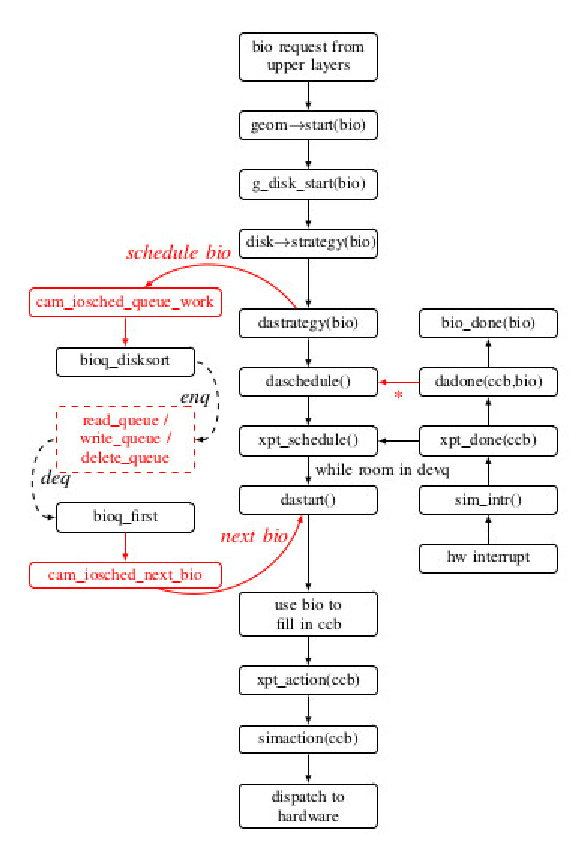
\includegraphics[scale=.7]{graph2.eps}
    \caption{A graph of the workflow done by the CAM scheduler. The red indicates what is different between CAM and the old default scheduler \cite{bsd2}.}
\end{figure}

A search for information on the CAM scheduler yields many results mentioning NetFlix. This is because NetFlix contributed to the development. With the old FreeBSD I/O scheduler, the read time for I/O requests was much too high on SSDs, as illustrated in the graph below. \\ \\

\begin{figure}[H]
\centering
    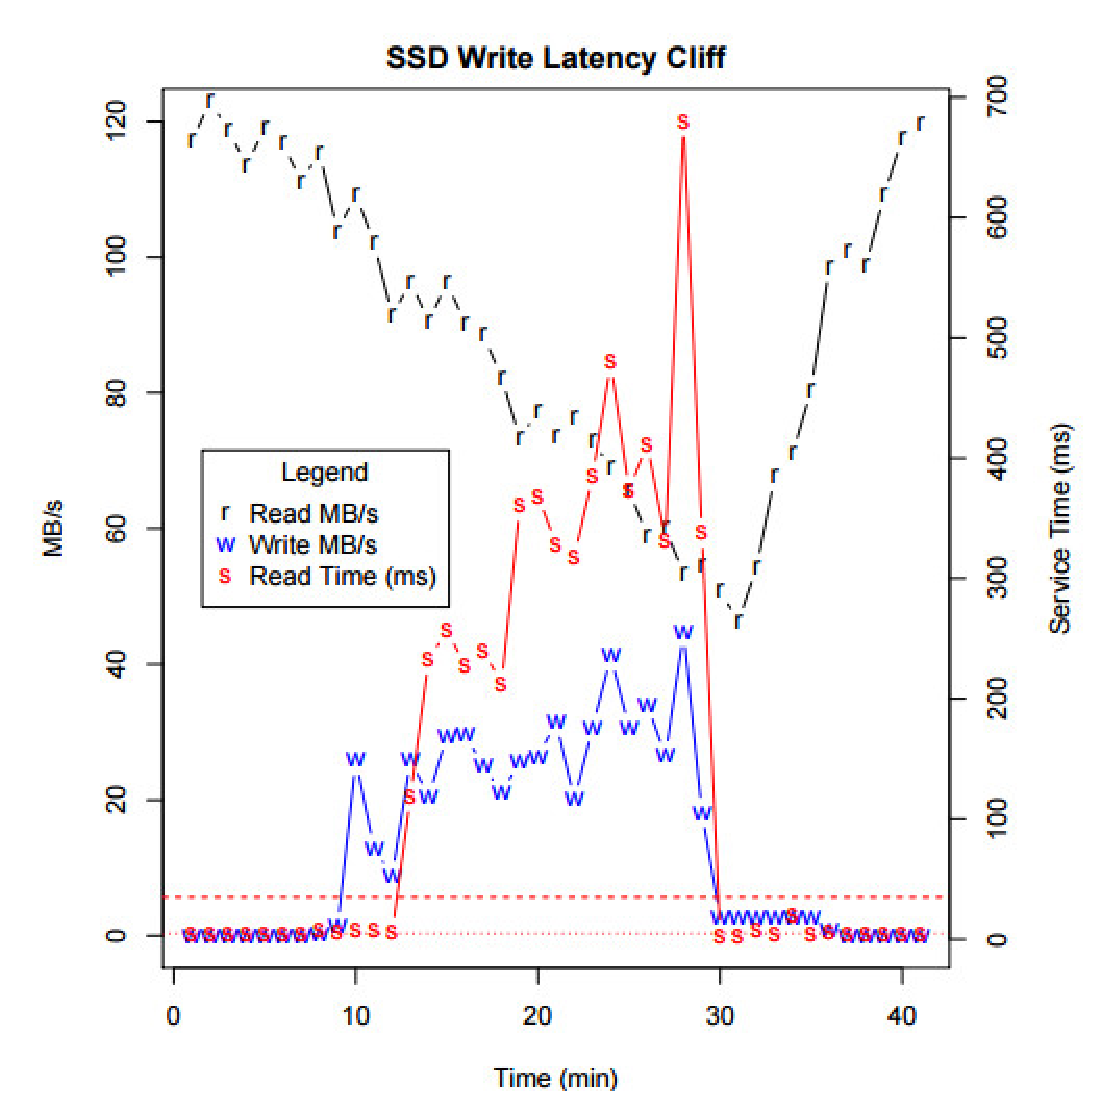
\includegraphics[scale=.85]{graph.eps}
    \caption{A graph of reads and writes done by the old default FreeBSD I/O scheduler. Note that the red line, read time, spikes heavily \cite{bsd2}.}
\end{figure}

\section{Windows}
In Windows, the I/O scheduling algorithms are referred to as 'strategies' and are divided into hierarchy prioritization and idle prioritization. There are only 5 priority levels, listen below, and they determine how I/O requests are scheduled \cite{winint}. \\ \\
\begin{tabular}{ | p{0.2\linewidth} |}
    \hline
    Critical\\ \hline
    High \\ \hline
    Normal \\ \hline
    Low \\ \hline
    Very low \\ \hline
\end{tabular} \\ \\ 

All requests that are of the 'very low' priority are scheduled via idle prioritization and the rest are scheduled via hierarchy prioritization. The default priority is 'normal'. Applications that do tasks in the background (e.g. Windows Defender) are generally assigned a priority of 'very low'. All requests made by the kernel have at least 'normal' priority, which is a concept called \textit{kernel bump} \cite{winint}.

Hierarchy prioritization has a simple underlying concept for scheduling. All 'critical' tasks must be dispatched before 'high' tasks, all 'high' tasks must be dispatched before 'normal' tasks, and all 'normal' tasks must be dispatched before 'low' tasks. Hierarchy prioritization has its own queue \cite{winint}.

Idle prioritization has its own queue as well. In general, tasks on the hierarchy prioritization's queue are dispatched first since their priorities are higher. Here, there is a very clear chance for starvation. As long as there is at least one request on the hierarchy prioritization's queue, requests on the idle prioritization's queue will starve. To avoid this, idle prioritization enforces at least one request on its queue is dispatched per unit of time (generally .5s). The ATA and USB port drivers use hierarchy prioritization and SCSI and storage port drivers use idle prioritization \cite{winint}. 

Cryptography in Windows can be done with the FileInfo API used with .NET. The methods \textit{Encrypt} and \textit{Decrypt} do what they say on the box \cite{wincrypt}. Entire volumes are encrypted and decrypted using BitLocker, which is included on Windows operating systems starting with Windows Vista \cite{wincrypt2}.

Overall, Windows has less variety when it comes to I/O scheduling algorithms and the scheduling algorithms appear to be fairly simple at a glance.


\newpage

\begin{thebibliography}{18}

\bibitem{linux1}
Love, R. \textit{Linux Kernel Development}. 2nd ed. Indianapolis, IN: Novell, 2005. Print.

\bibitem{bsd1}
Losh, W. M. "CAM I/O Scheduler." Warner's Boring FreeBSD Page. FreeBSD, 15 Apr. 2015. Web. 17 May 2017.
Available: \url{https://people.freebsd.org/~imp/asiabsdcon2015/iosched-slides.pdf}

\bibitem{bsd2}
Losh, W. M. "I/O Scheduling in FreeBSD’s CAM Subsystem." Warner's Boring FreeBSD Page. FreeBSD, 2015. Web. 18 May 2017. \\
Available: \url{https://people.freebsd.org/~imp/bsdcan2015/iosched-v3.pdf}

\bibitem{winint}
Russinovich, M. E., D. A. Solomon, and A. Ionescu. \textit{Windows Internals}. Redmond (Wash.): Microsoft, 2012. Print.

\bibitem{wincrypt}
"FileInfo Methods." .NET Development. Microsoft, n.d. Web. 18 May 2017. \\
Available: \url{https://msdn.microsoft.com/en-us/library/system.io.fileinfo_methods(v=vs.110).aspx}

\bibitem{wincrypt2}
Paul, I. "A Beginner's Guide to BitLocker, Windows' Built-in Encryption Tool." PCWorld. PCWorld, 01 Aug. 2016. Web. 18 May 2017. \\
Available: \url{http://www.pcworld.com/article/2308725/encryption/a-beginners-guide-to-bitlocker-windows-built-in-encryption-tool.html}

\end{thebibliography}


\end{document}
